\documentclass{article}

\usepackage{listings}
\usepackage[T1]{fontenc}
\usepackage[letterpaper, margin=1in]{geometry}
\usepackage{graphicx}
\usepackage{multicol}
\usepackage{xcolor}
\usepackage{enumitem}
\usepackage{moresize}
\usepackage{mathtools}
\usepackage{array}
\graphicspath{{./}}

\pagenumbering{gobble}

\colorlet{keyword}{blue!100!black!80}
\colorlet{comment}{green!30!black!100}
\definecolor{string}{gray}{0.3}
\definecolor{ndkeyword}{HTML}{FF1493}
\definecolor{lightergray}{gray}{0.9}

\setlist[enumerate]{noitemsep, topsep=0pt}
\setlist[itemize]{noitemsep, topsep=0pt}

\newcommand{\ti}[1]{\hangindent=0.25in\noindent\begin{scriptsize}\textbf{#1:}\end{scriptsize}}
\newcommand{\chaptertitle}[1]{\noindent\begin{normalsize}\textit{\textbf{#1}}\end{normalsize}}
\newcommand{\hi}{\setlength\parindent{0.25in}\indent\hangindent=0.75in}
\newcommand{\ttt}[1]{\texttt{#1}}
\newcommand{\ra}{$\rightarrow$ }
\newcommand{\sa}{\textbf{Answer: }}
\DeclarePairedDelimiter{\ceil}{\lceil}{\rceil}

\begin{document}

	\begin{normalsize}
	\noindent \textbf{Computer System Design Test \#2 Note Sheet}
	\end{normalsize}
	
	\begin{scriptsize}
	\begin{multicols*}{2}
		
		\chaptertitle{ISA}
		
		\ti{CPU and ISA versions}
		
			\noindent \begin{tabular}{m{1.65cm}|c|c|c}
				Processor & Address Bus & Data Bus & Control Bus \\ \hline
				8086 & 20 bit & 16 bit & \\\hline
				8088 & 20 bit & 8 bit & \\\hline
				80286 & 24 bit & 16 bit & \\\hline
				80386 \newline 80486 \newline Pentium I \newline Pentium II \newline Pentium III& 32 bit & 32 bit & \\\hline
				Pentium IV & 32/36 bit & 32 bit & \\\hline
				Pentium D & 32/36 bit & 32/64 bit & \\\hline
			\end{tabular}
			
		\ti{Address Time} Driven by internals of the processor, the PCLK cycle where address is output (Ts)
		
		\ti{Data Time} Driven by internals of processor, the PCLK cycle(s) where data is sent/recieved (Tc)
		
		\ti{Wait State} Driven by ICs outside the processor when >1 PCLK is needed to complete work
		
			\hi \ti{Ready\_n} Signal that allows external devices to insert wait states
		
		\ti{Address Space, IO Space}
		
		\noindent\begin{tabular}{cc}
			Memory map & I/O Map \\
			\begin{tabular}{|m{2.2cm}|}
				\hline
				64KB \newline Boot ROM \\ \hline
				64KB \newline Option ROM \\ \hline
				128KB \newline Device ROM \\ \hline
				128KB \newline Video Memory \\ \hline
				640KB \newline Conventional Memory \\ \hline
			\end{tabular} &
			\begin{tabular}{|c|c|}
				\hline
				I/O Sub Range & \\ \hline
				0000h to 001Fh & DMAC1CS\# \\ \hline
				0020h to 003Fh & PIC1CS\# \\ \hline
				0040h to 005Fh & PITCS\# \\ \hline
				0060h to 007Fh & MISC1CS\# \\ \hline
				0080h to 009Fh & MISC2CS\# \\ \hline
				00A0h to 00BFh & PIC2CS\# \\ \hline
				00C0h to 00DFh & DMAC2CS\# \\ \hline
				00E0h to 00FFh & NCPCS\# \\ \hline
			\end{tabular}
		\end{tabular}
		
		\ti{Address Decoders} Typically made using a MUX, unique address lines as the select lines and M/IO\# going into the enable
		
		\ti{Register}
		
			\hi\ti{AX} General Purpose Register (GPR), ALU input and the output
			
			\hi\ti{BX} GPR, ALU input
			
			\hi\ti{CX} GPR or the loop index
			
			\hi\ti{DX} GPR, holds values in fast memory
			
			\hi\ti{CS} Code Seg Reg, holds start of code seg
			
			\hi\ti{DS} Data Seg Reg, points to user variables
			
			\hi\ti{SS} Stack Seg Reg, start of stack
			
			\hi\ti{ES} Extrasegment Reg, stores an extra segment
			
			\hi\ti{IP} Instruction Pointer, inside the current CS
			
			\hi\ti{SP} Stack pointer, inside the current SS
		 
		\ti{Address Generation from Registers} Shift CS left by 4, add IP. Carry bit is saved in >286
		
		\ti{Little-Endian Byte Ordering} LSB at the lowest address
		
		\ti{Extended Memory} Memory past 1Meg, accessable by a 286 in real mode (carry out of CS+IP is 1)
		
		\ti{Cardinal Rules}
		
		\begin{enumerate}[noitemsep,nolistsep]
			\item In any system based on the X86 microprocessors, every memory and I/O storage location contains 1 byte, no more or less.
			\item Every memory and I/O address is considered to be either an even or odd address
			\item When the 80286 microprocessor reads from or writes to an even address, the data is transferred over the lower data path. Upper path for an address.
		\end{enumerate}
		
		\ti{Control Signals}
		
			\hi\ti{\underline{Processor Signals}}
			
			\hi\ti{BHE\#} Byte High Enable, D15-D8 are used in transfer
			
			\hi\ti{A0} Odd (1) or even (0) address accessed
			
			\hi\begin{tabular}{lll|m{1.5cm}|m{1.5cm}}
				M/IO\# & S1\# & S0\# & Cycle Type & ISA \newline Line Assert\\ \hline
				0 & 0 & 0 & Interrupt ack. & none\\
				0 & 0 & 1 & I/0 read & IOWC\# \\
				0 & 1 & 0 & I/0 write & IORC\# \\
				1 & 0 & 0 & Halt\newline shutdown & none\\
				1 & 0 & 1 & Mem read & (S)MWTC\#\\
				1 & 1 & 0 & Mem write & (S)MRDC\#
			\end{tabular}
			
			\hi\ti{\underline{Bus Signals}}
			
			\hi\ti{Upper Enable} Read the name
			
			\hi\ti{Lower Enable} Read the name
			
			\hi\ti{Copy Enable} copy from upper half to lower
			
			\hi\ti{DT/R\#} Data transmit/recieve, tell tranceivers what direction to allow flow
			
			\hi\ti{Copy Enable} turns on/off steering logic
			
			\hi\ti{SA0} Same as A0
		
		\ti{Bus Mastering}
		
			\hi\ti{HOLD} input to the processor requesting the processor stop driving the bus
			
			\hi\ti{HLDA} output from the process indicating the bus is now undriven
			
			\hi\ti{LOCK\#} output from processor, set by software indicating the current instruction set is being executed atomically
		
		\ti{Power on Reset} Holds the processor in reset for a certain amount of time after turn on
		
		\ti{First Bus Cycle} CS and IP set to F000h and FFF0h respectively. First instruction from top 16 bytes of memory space.
		
		\ti{Address Latch} see SA
		
		\ti{LA vs. SA}
		
			\hi \ti{LA} Latchable address lines, on the 16 bit half, updated before address phase to allow mem cards to perform bank selection
			
			\hi\ti{SA} Latched version of the processor address lines on lower half. Presented during address phase, held until next address phase.
			
			\hi\ti{ALE} Add. Latch En., indicates address lines valid
		
		\ti{Bus Steering Logic} routes data from up half to low half, needed for 8 bit compatibility
		
			\hi\ti{Data Bus Transceivers} half duplex latches that control data flow direction on up/low halves of bus
		
		\ti{Stretching the Transfer Time (Wait States)} For operations that require more than 1 PCLK cycle
		
			\hi\ti{Default Wait States / Ready Timers}
			
			\hi\begin{tabular}{lclc}
				16-bit RAM & 1 & 8-bit RAM & 4 \\
				16-bit I/0 & 1 & 8-bit I/0 & 4 \\
			\end{tabular}
			
			\hi\ti{NOWS\#} reduces the number of wait states to 0 for 16-bit, 1 for 8-bit
			
			\hi\ti{CHRDY\#} card forces extra wait states by deasserting 
		
		\ti{Protected Mode vs. Real Mode}
		
			\hi\ti{Protected Mode} Only have access to 1M of memory, compatible with 8086
			
			\hi\ti{Real Mode} Have acces to 1M + the extended memory, compatible with 80286+
		
		\ti{ISA Bus Structure} 
		
		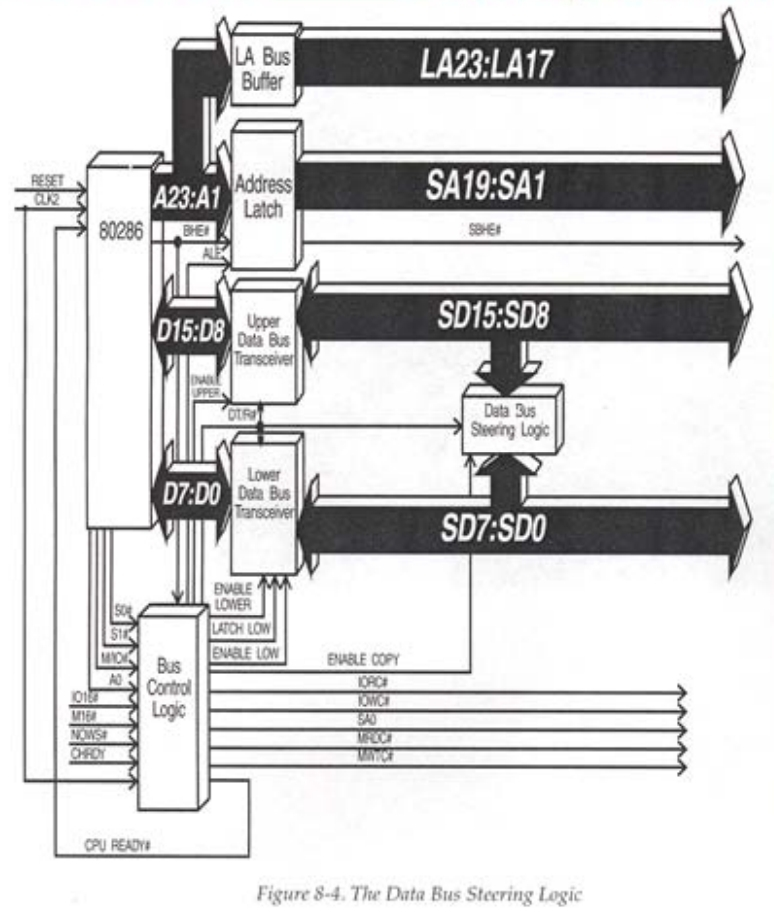
\includegraphics[width=0.5\linewidth]{isaStruct}
		
		\ti{ISA Bus Cycle Timing}
		
			\hi\ti{BCLK} Derived from input clock, designed to be 8MHz
		
		\ti{Device Size Indication}
		
			\hi\ti{M16\#} signals whether a device is capable of 16 bit memory transactions. 0 = 8 bit device. 1 = 16 bit
			
			\hi\ti{I016\#} Sames as M16\#, but for I/O devices
		
		\ti{ISA Bus Cycles}
		
		\ti{Detailed view of 286 Bus Cycle}
		
		\ti{Detailed View of ISA Bus Cycle}
		
		
	\end{multicols*}
	\end{scriptsize}
\end{document}